\documentclass[conference]{IEEEtran}

\usepackage{amsmath,amssymb,amsfonts,latexsym}
\usepackage{graphicx,psfrag}
\usepackage{booktabs}
\usepackage{url}
\IEEEoverridecommandlockouts
\hyphenation{op-tical net-works semi-conduc-tor auto-en-coder}

\begin{document}

\title{Market Regime Detection Using Autoencoders and\\ Principal Component Analysis}
\author{Eleni Tsaousi, Adene Dinoshi, Harjot Singh$^{\diamond}$
\thanks{$\diamond$ Investments -- Selected Quantitative Tools, University of Zurich. Supervisor: Matthias Feiler.}}
\maketitle

\begin{abstract}
Financial markets transition between distinct regimes characterized by varying
levels of volatility, economic conditions, and investor sentiment. We
investigate the use of autoencoders for unsupervised market regime detection in
financial time series. Using financial and macroeconomic indicators arranged
into rolling windows, we learn a 16-dimensional latent representation with a
feed-forward autoencoder and apply K-Means clustering to identify four market
regimes. As a benchmark, we compare the result with a Principal Component
Analysis (PCA) projection of identical dimensionality. Both methods uncover
interpretable market structures, but they agree only moderately (adjusted Rand
index $0.52$), indicating that the autoencoder captures nonlinear structure that
linear PCA cannot reproduce in 16 components. To assess whether the regimes
carry economic value, we construct a simple regime-conditioned long/short
trading rule, fixed from training data and evaluated out of sample. The rule is
profitable and economically sensible in sample but fails to generalize to the
test period (Sharpe ratio $-0.28$ versus a buy-and-hold benchmark), indicating
that, in its current form, the regime signal is not yet a reliable
stand-alone basis for investment decisions.
\end{abstract}

\section{Introduction}

Financial markets are dynamic systems that continuously evolve in response to
economic, political, and behavioral factors. Over time, markets transition
between different states, commonly referred to as \textit{market regimes}. These
regimes are characterized by distinct patterns in returns, volatility, interest
rates, inflation, and other macroeconomic indicators. Examples include periods
of sustained growth and optimism (bull markets), prolonged declines (bear
markets), high-volatility environments, and crisis periods associated with
economic stress.

Identifying such regimes is an important task in quantitative finance.
Knowledge of the prevailing market environment can support portfolio
allocation, risk management, asset pricing, and investment decision-making.
Traditional approaches to regime detection rely on predefined economic
indicators, statistical models such as Hidden Markov Models~\cite{hamilton1989new,ang2002regime}, or dimensionality
reduction techniques. One of the most widely used methods is Principal Component
Analysis (PCA)~\cite{stock2002forecasting}, which projects high-dimensional financial data onto a small set
of linear factors. While PCA is effective and interpretable, its linear nature
may limit its ability to capture the nonlinear relationships often present in
financial markets.

Recent advances in representation learning offer new ways to uncover hidden
structure directly from data~\cite{bengio2013representation}. Autoencoders, in particular, learn compact latent
representations by compressing inputs through a bottleneck and reconstructing
them~\cite{hinton2006reducing,rumelhart1986learning}. This allows them to capture nonlinear dependencies that are not accessible
to linear methods, providing a data-driven route to identifying market
structure without relying solely on predefined assumptions.

\subsection{Objective}

The primary objective of this project is to investigate whether an autoencoder
can learn meaningful latent representations of financial market behavior, and
whether these representations can be used to identify distinct market regimes.
Financial and macroeconomic indicators are transformed into rolling windows and
used as inputs to the autoencoder. The resulting latent representations are
clustered to detect groups of observations corresponding to different market
environments. To assess the value of nonlinear representation learning, the
autoencoder is benchmarked against PCA under an identical dimensionality and
clustering setup, isolating the effect of the representation method itself.

\subsection{Contributions}

This project makes four contributions. First, it develops an autoencoder-based
framework for extracting latent representations from financial time-series
windows. Second, it applies K-Means clustering to the learned representations to
identify distinct market regimes in a fully unsupervised manner. Third, it
compares the autoencoder representation against a PCA baseline under a common
experimental setup, quantifying their agreement with the adjusted Rand index and
normalized mutual information. Finally, it provides visualizations and economic
interpretations of the discovered regimes, linking them to underlying market and
macroeconomic conditions.

\section{Related Work}

\textit{Market regime detection} aims to identify periods with distinct market
dynamics, such as varying levels of volatility, trend, and risk. Established
approaches include statistical models, Hidden Markov Models~\cite{hamilton1989new,nystrup2017regime}, clustering
techniques~\cite{procacci2021portfolio}, and factor-based methods~\cite{fama1993common}.

\textit{Dimensionality reduction in finance} is widely used to uncover hidden
structure in high-dimensional datasets. PCA is among the most common methods for
extracting dominant market factors~\cite{stock2002forecasting,guidolin2007asset} and is a natural linear baseline for this
study.

\textit{Autoencoders for financial time series} extend dimensionality reduction
to the nonlinear setting. Unlike PCA, autoencoders can model nonlinear
relationships and have been applied to anomaly detection, feature extraction,
and representation learning in financial applications~\cite{kaya2020unsupervised}.

\section{Data and Preprocessing}

\subsection{Dataset}

The study uses the course market dataset (\texttt{market\_data.xlsx}, US sheet),
consisting of 30 financial and macroeconomic indicators observed at weekly
frequency from 1988 to 2026. The indicators span equity and asset returns,
interest rates and yields, valuation ratios, and macroeconomic aggregates such
as inflation, unemployment, and money supply.

\subsection{Transformations and Splits}

Eight price and index columns are non-stationary as raw levels (augmented
Dickey--Fuller~\cite{dickey1979distribution} $p \approx 0.18$--$1.0$) and are converted to log-returns~\cite{campbell1997econometrics}, after
which all eight become strongly stationary ($p < 0.0001$). The data is then
split chronologically using forward chaining~\cite{lopez2018advances}, with the training partition being
the oldest and the test partition the most recent, so that no future information
leaks into the past:
\begin{itemize}
  \item train: 1988--2014 (70\%),
  \item validation: 2014--2020 (15\%),
  \item test: 2020--2026 (15\%).
\end{itemize}
A \texttt{StandardScaler} is fitted on the training data only and applied to all
partitions, ensuring zero mean and unit variance on the training set and
avoiding leakage.

\subsection{Rolling Windows}

The standardized series are transformed into overlapping sliding windows of 26
weeks (approximately six months, stride one), built per split so that no window
crosses a partition boundary. A 26-week horizon is long enough to smooth
single-week noise yet short enough to capture a regime change within a quarter
or two. Each window flattens 26 time steps $\times$ 30 features into a
780-dimensional input vector. The resulting tensors have shapes
$(1365, 26, 30)$, $(273, 26, 30)$, and $(273, 26, 30)$ for train, validation,
and test respectively.

\section{Methodology}

This study adopts an unsupervised framework for identifying market regimes.
Because regimes are not directly observable, the objective is to uncover latent
structure that may correspond to different economic and market environments. The
framework has four stages: windows of financial and macroeconomic data are
compressed into a low-dimensional representation using both an autoencoder and
PCA; the representations are clustered with K-Means; and the resulting clusters
are interpreted as market regimes and analyzed from a financial perspective.

\begin{figure}[t]
  \centering
  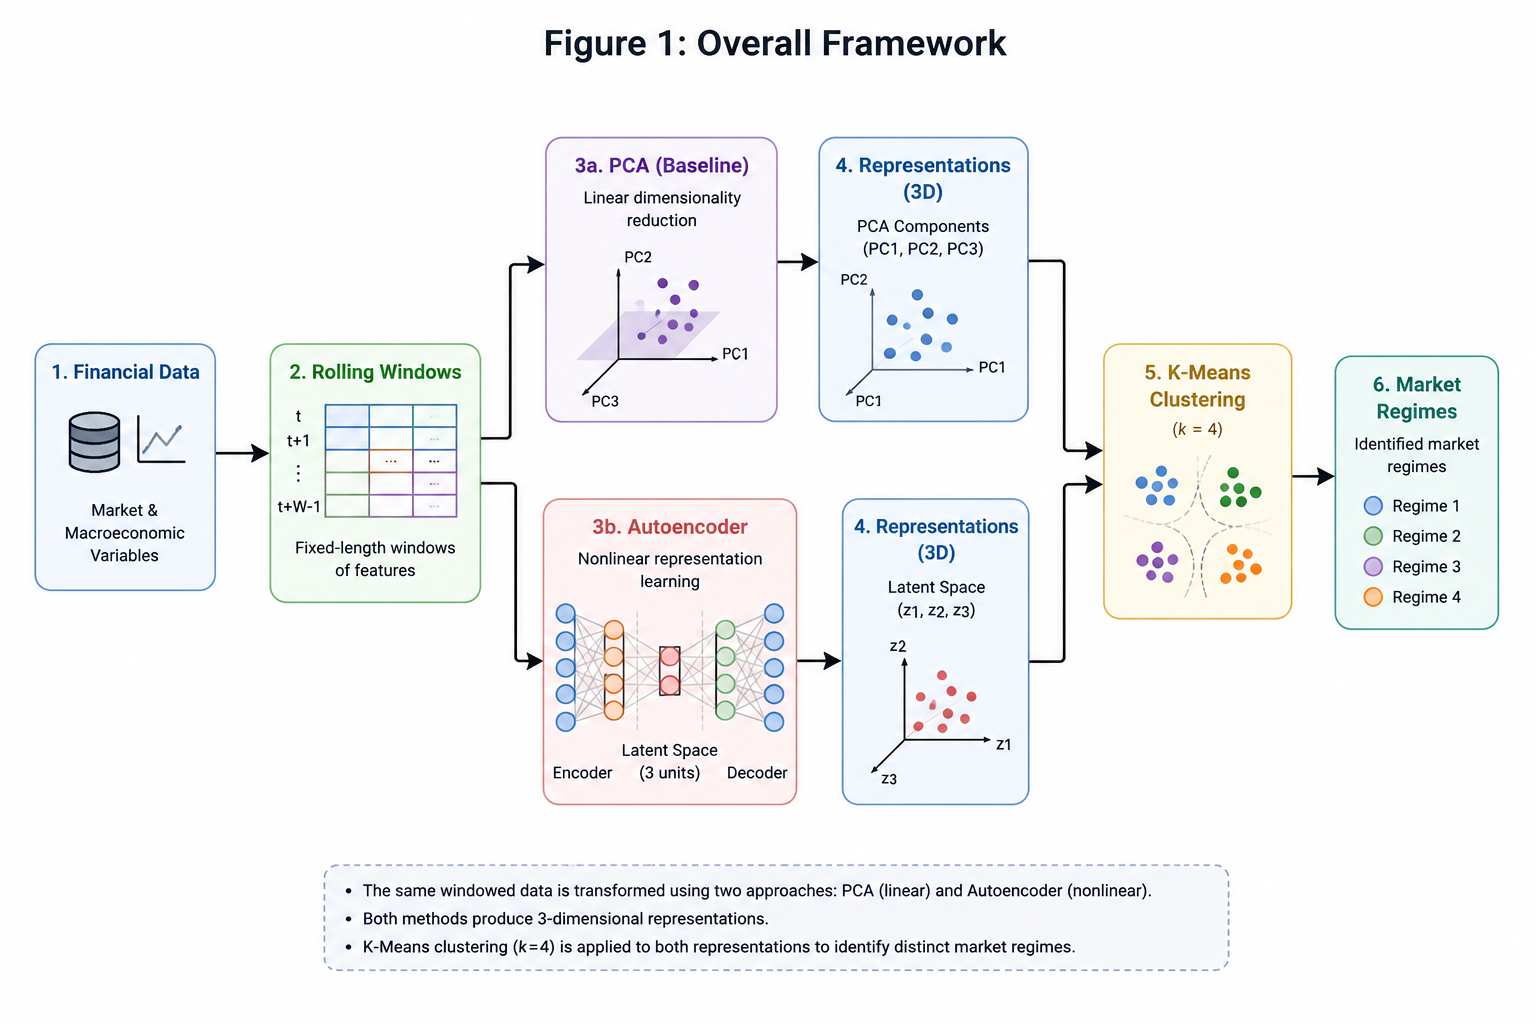
\includegraphics[width=0.9\columnwidth]{framework.png}
  \caption{Overall framework of the market regime detection pipeline}
  \label{fig:framework}
\end{figure}

\subsection{Autoencoder Architecture}

The primary model is a feed-forward autoencoder implemented in PyTorch~\cite{paszke2019pytorch}. An
autoencoder consists of an encoder that maps the input to a compressed latent
code and a decoder that reconstructs the input from that code. By minimizing the
reconstruction error, the network is forced to retain the most informative
aspects of the data. The architecture is
\begin{center}
Input(780) $\rightarrow$ Dense(256) $\rightarrow$ ReLU $\rightarrow$ Dense(64)
$\rightarrow$ ReLU $\rightarrow$ Latent(16) $\rightarrow$ Dense(64) $\rightarrow$
ReLU $\rightarrow$ Dense(256) $\rightarrow$ ReLU $\rightarrow$ Output(780).
\end{center}
The bottleneck is a deliberate design choice. If the latent space were as large
as the input, the network could memorize the data without extracting structure.
Restricting it to 16 dimensions forces the model to compress information and
learn the most important characteristics of market behavior while mitigating
the severe mode collapse often seen in overly narrow architectures.

\begin{figure*}[t]
  \centering
  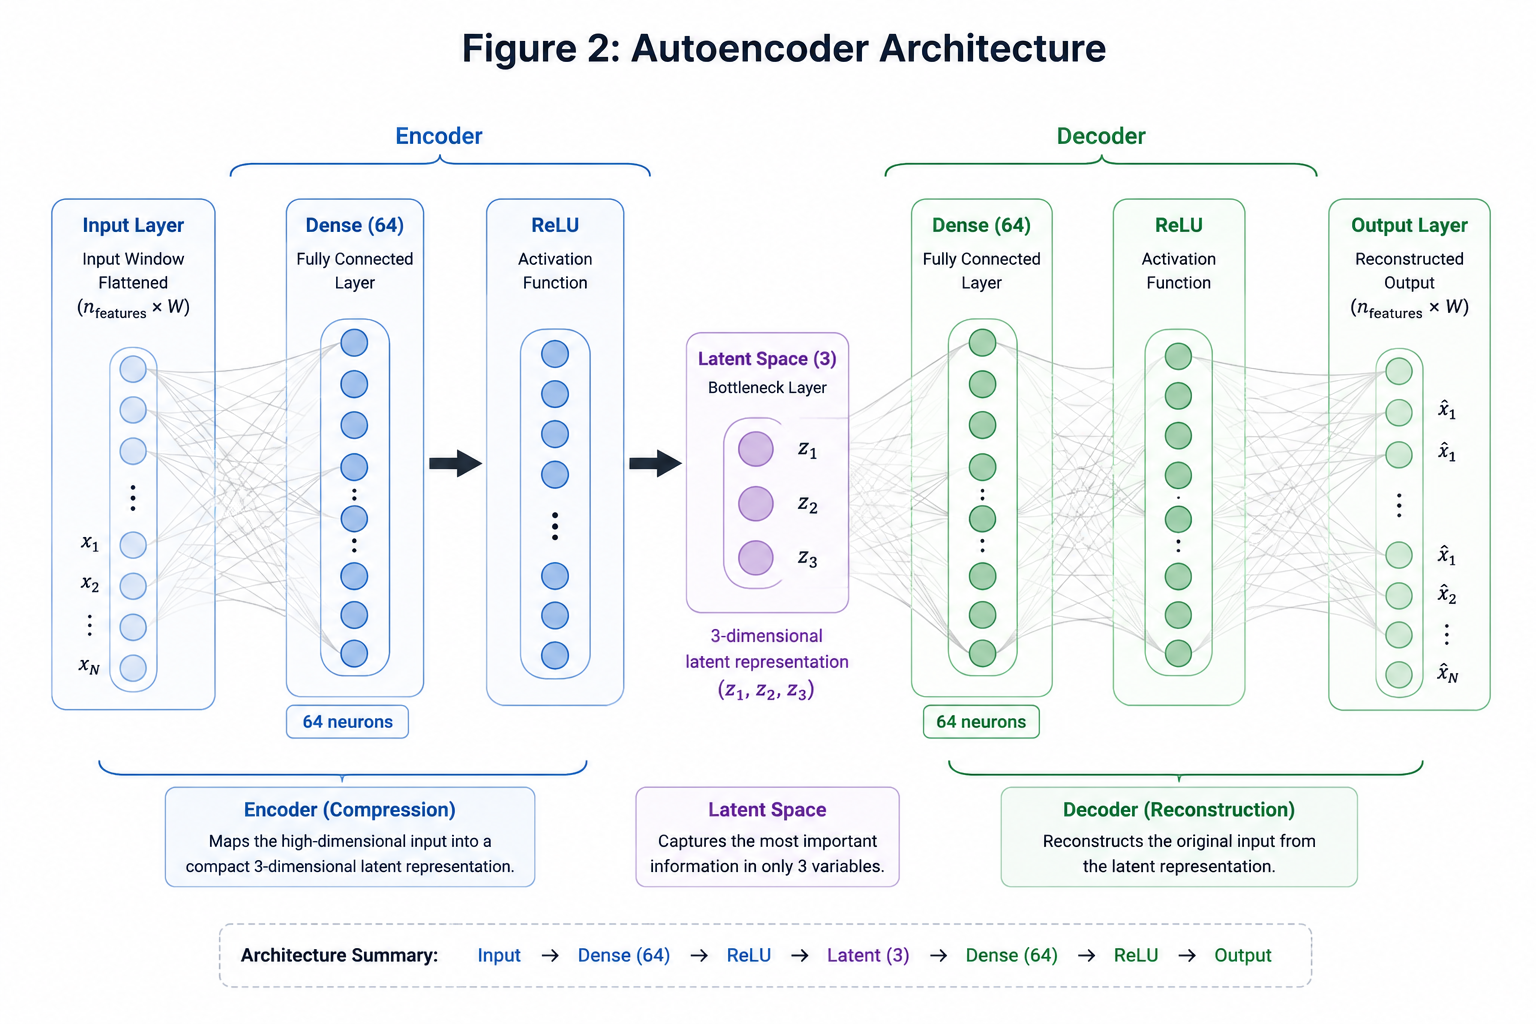
\includegraphics[width=\textwidth]{autoencoder_architecture.png}
  \caption{Architecture of the autoencoder used for latent representation
  learning: a two-layer encoder ($256 \rightarrow 64$ units) compresses the
  flattened window into a 16-dimensional latent space $(z_1, \ldots, z_{16})$,
  which a symmetric two-layer decoder ($64 \rightarrow 256$ units) reconstructs
  back to the original dimensionality.}
  \label{fig:autoencoder_architecture}
\end{figure*}

\subsection{Training Procedure}

The autoencoder is trained on the training partition by minimizing the mean
squared reconstruction error,
\[
\mathrm{MSE} = \frac{1}{n}\sum_{i=1}^{n}(x_i - \hat{x}_i)^2,
\]
where $x_i$ is the original input and $\hat{x}_i$ its reconstruction.
Optimization uses Adam~\cite{kingma2014adam} on mini-batches. Because financial data is noisy and
prone to overfitting, several regularization mechanisms are applied: weight
decay penalizes large parameters, a validation set monitors generalization, and
early stopping retains the model with the lowest validation loss. The main
hyperparameters are summarized in Table~\ref{tab:hyperparameters}.

\begin{table}[h]
\centering
\caption{Model configuration and training hyperparameters.}
\label{tab:hyperparameters}
\begin{tabular}{lc}
\toprule
Parameter & Value \\
\midrule
Hidden dimensions & 256, 64 \\
Latent dimension & 16 \\
Optimizer & Adam \\
Loss function & MSE \\
Weight decay & $5\times10^{-4}$ \\
Early stopping patience & 40 \\
Number of clusters & 4 \\
\bottomrule
\end{tabular}
\end{table}

\subsection{PCA Baseline}

PCA is used as a linear benchmark. It identifies orthogonal directions of
maximum variance and projects observations onto a lower-dimensional subspace.
For comparability, PCA is configured to produce 16 components, matching the
autoencoder latent dimensionality, so that performance differences can be
attributed primarily to the representation method rather than to dimensionality.
PCA is fitted on the training windows only and applied to all partitions.

\subsection{Clustering and Regime Identification}

After dimensionality reduction, regimes are identified with K-Means~\cite{lloyd1982least}. The latent
variables are standardized so each dimension contributes equally, and the
algorithm partitions observations into four clusters. To avoid leakage, K-Means
is fitted on the training latent vectors only and then used to assign regimes to
validation and test. Each cluster is interpreted as a candidate market regime
and analyzed with respect to the behavior of market and macroeconomic variables
within it.

The choice of four clusters is driven primarily by economic interpretability and
parsimony rather than by an internal cluster-validity optimum. On the training
latent space the silhouette score rises monotonically with $K$ (from $0.25$ at
$K=2$ to $0.35$ at $K=8$) and the inertia elbow is shallow, so the standard
metrics do not single out a particular $K$. We deliberately favor a small number
of regimes: four states map cleanly onto recognizable macro-financial conditions
(easing, inflationary, stress, and a transitional baseline), whereas larger $K$
fragments the space into clusters that gain marginal silhouette but lose economic
meaning and out-of-sample stability.

\section{Experiments and Results}

\subsection{Autoencoder Reconstruction}

The autoencoder is trained for up to 200 epochs with early stopping. Training
reduces the reconstruction loss to roughly $0.30$ on the training set, about a
$70\%$ improvement over a naive baseline that predicts the per-feature training
mean (loss $\approx 1.00$), confirming that the model learns genuine structure
rather than a trivial solution. Table~\ref{tab:recon} reports the reconstruction
loss by split.

\begin{table}[h]
\centering
\caption{Autoencoder reconstruction loss (MSE) by split.}
\label{tab:recon}
\begin{tabular}{lc}
\toprule
Split & Reconstruction loss \\
\midrule
Train & 0.299 \\
Validation & 0.611 \\
Test & 1.205 \\
\bottomrule
\end{tabular}
\end{table}

The substantially higher test loss is expected: the test partition (2020--2026)
is the most recent and includes market conditions --- the post-2020 inflation
and rate-hike cycle --- that differ from the training period. We interpret this
as evidence of a possible regime shift rather than as a model failure.

\subsection{Latent-Dimension Ablation}
\label{sec:ablation}

To justify the 16-dimensional bottleneck, we retrain the autoencoder at several
latent widths under identical settings and report both reconstruction quality and
the number of distinct regimes populated in each split when K-Means ($K=4$) is fit
on the training latent vectors (Table~\ref{tab:ablation}).

\begin{table}[h]
\centering
\caption{Latent-dimension ablation. Reconstruction MSE on train and test, and the
number of the four K-Means regimes that are actually populated in each split.}
\label{tab:ablation}
\begin{tabular}{cccc}
\toprule
Latent dim & Train MSE & Test MSE & Regimes (train/val/test) \\
\midrule
2  & 0.391 & 1.608 & 4 / 2 / 4 \\
3  & 0.389 & 1.561 & 4 / 2 / 4 \\
8  & 0.303 & 1.491 & 4 / 2 / 3 \\
\textbf{16} & \textbf{0.303} & \textbf{1.197} & 4 / 2 / 3 \\
32 & 0.313 & 1.280 & 4 / 3 / 4 \\
\bottomrule
\end{tabular}
\end{table}

Two observations follow. First, reconstruction improves sharply from the narrow
2--3 dimensional bottlenecks (train MSE $\approx 0.39$, test MSE $\approx 1.6$) to
eight dimensions, then plateaus; the 16-dimensional model attains the lowest test
reconstruction loss ($1.197$), while widening further to 32 dimensions slightly
degrades it, indicating mild overfitting. This is our primary reason for adopting
16 dimensions. Second, and more revealing, out-of-sample regime coverage does
\emph{not} improve with capacity: the validation period populates only two of the
four regimes at almost every latent width. The collapse therefore reflects a
genuine structural shift in the validation and test periods rather than an
insufficient bottleneck --- a point we return to when the trading rule fails out
of sample (Section~\ref{sec:strategy}).

\subsection{PCA versus Autoencoder Agreement}

16 principal components explain $70.8\%$ of the training variance ($10$
components: $67.2\%$; $20$: $72.7\%$; $50$: $82.4\%$), meaning a 16-dimensional
linear projection captures a substantial portion of the variance the features carry. The
autoencoder compresses into the same 16 dimensions nonlinearly. Agreement
between the two regime assignments, measured on the full dataset, is
\[
\mathrm{ARI} = 0.515, \qquad \mathrm{NMI} = 0.577,
\]
which is moderate: the adjusted Rand index~\cite{hubert1985comparing} and normalized mutual
information~\cite{vinh2010information} indicate the methods share substantial structure but differ in
boundary placement, consistent with the autoencoder capturing nonlinear patterns
that PCA cannot represent even in 16 components.

\begin{figure}[t]
  \centering
  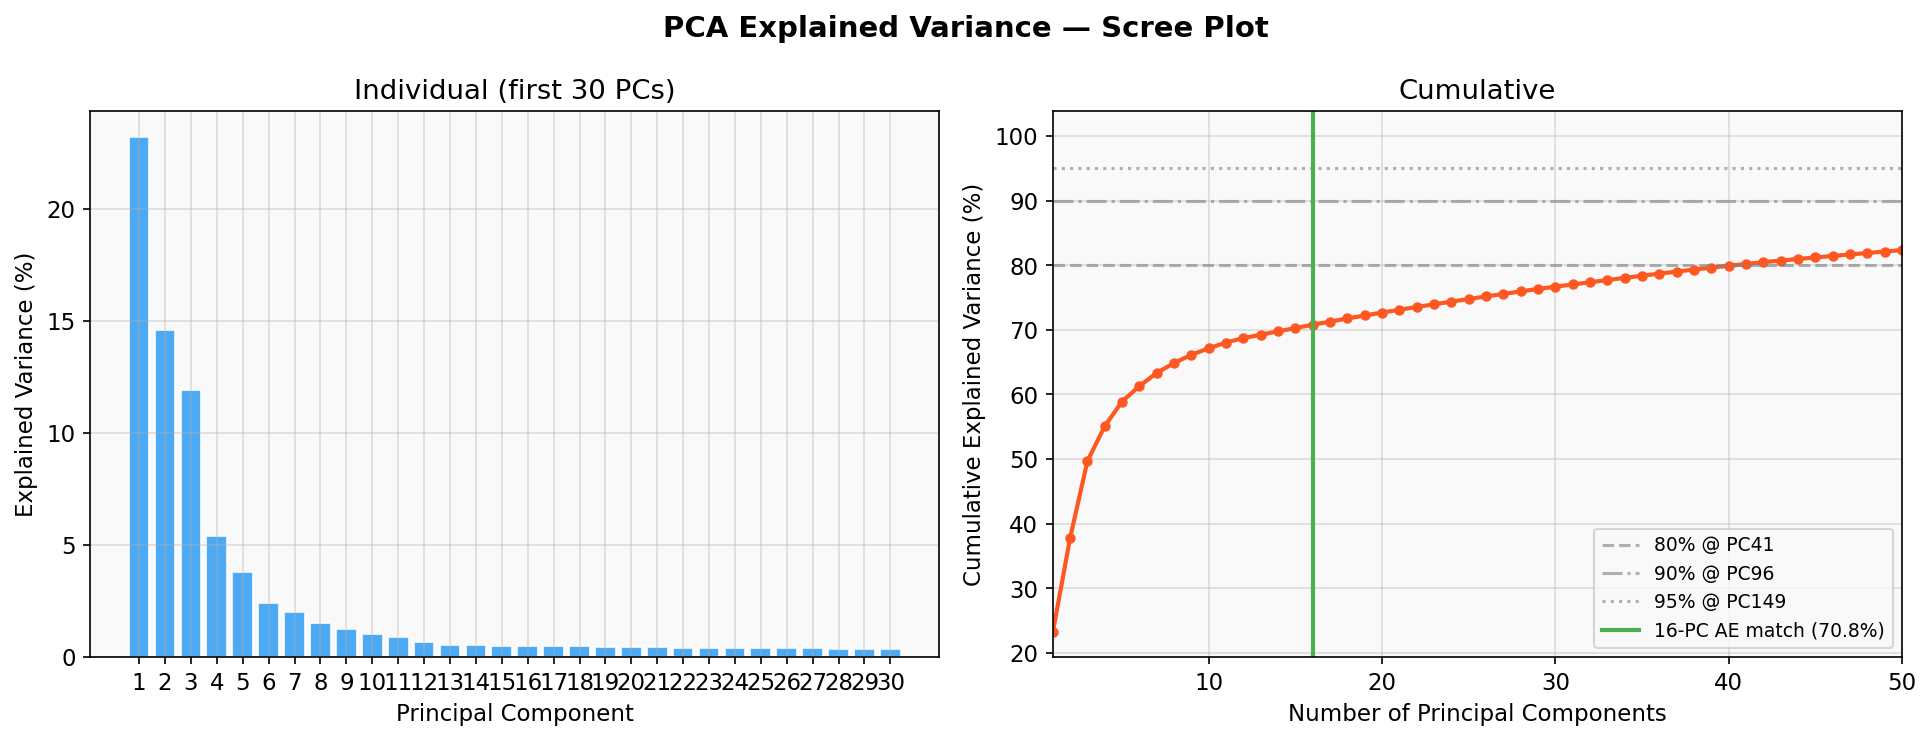
\includegraphics[width=\columnwidth]{01_scree_plot.png}
  \caption{PCA explained variance. 16 components retain $70.8\%$ of the
  training variance, motivating the wider bottleneck.}
  \label{fig:scree}
\end{figure}

\begin{figure}[t]
  \centering
  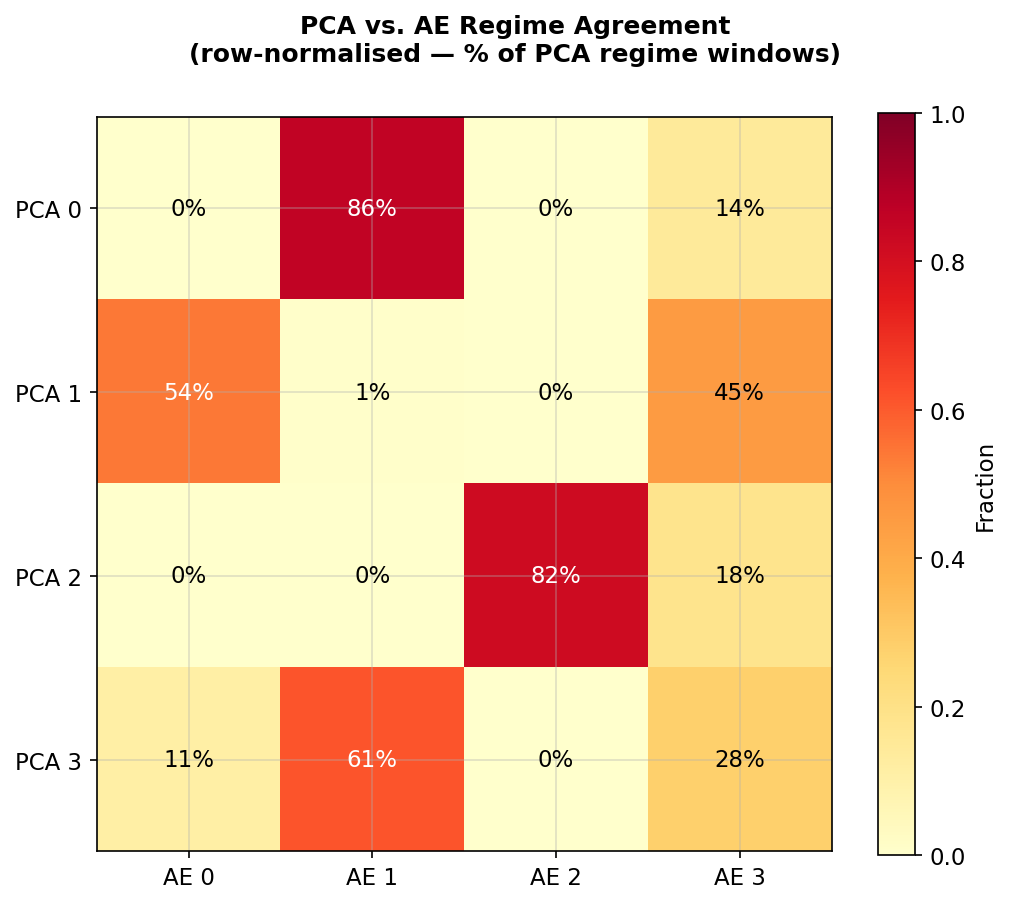
\includegraphics[width=\columnwidth]{07_regime_agreement_heatmap.png}
  \caption{Row-normalized agreement between PCA and autoencoder regime labels.
  Off-diagonal mass reflects the moderate ARI/NMI.}
  \label{fig:heatmap}
\end{figure}

\subsection{Market Regime Analysis}

Table~\ref{tab:regimes} summarizes the four PCA regimes on the training set
together with their dominant standardized features and a suggested economic
label. The labels are derived from feature profiles and require domain
validation before being treated as final.

\begin{table*}[t]
\centering
\caption{PCA market regimes (training set): size, dominant standardized features, and suggested interpretation.}
\label{tab:regimes}
\begin{tabular}{cll}
\toprule
Regime & Dominant features & Suggested interpretation \\
\midrule
0 (26.6\%) & 2Y yield $-1.17$, short rate $-1.15$, 10Y yield $-1.11$ & low volatility, falling long rates \\
1 (34.0\%) & CAPE $+1.08$, employment $+0.97$, real rate $+0.91$ & mixed / transitional \\
2 (27.3\%) & CPI $+1.25$, dividend yield $+1.19$, 10Y yield $+1.13$ & inflationary pressure, rising long rates \\
3 (12.1\%) & yield-spread stress $+1.94$, unemployment $+1.93$, GDP $-1.58$ & high volatility, elevated unemployment \\
\bottomrule
\end{tabular}
\end{table*}

Regime 3 is the smallest and most distinct, combining the highest unemployment,
the lowest GDP, and elevated volatility; it is the strongest candidate for a
``crisis'' label, pending a cross-check against known recession dates. Regime 1
is the largest and most diffuse, consistent with a normal-market baseline rather
than a sharply defined state.

\begin{figure*}[t]
  \centering
  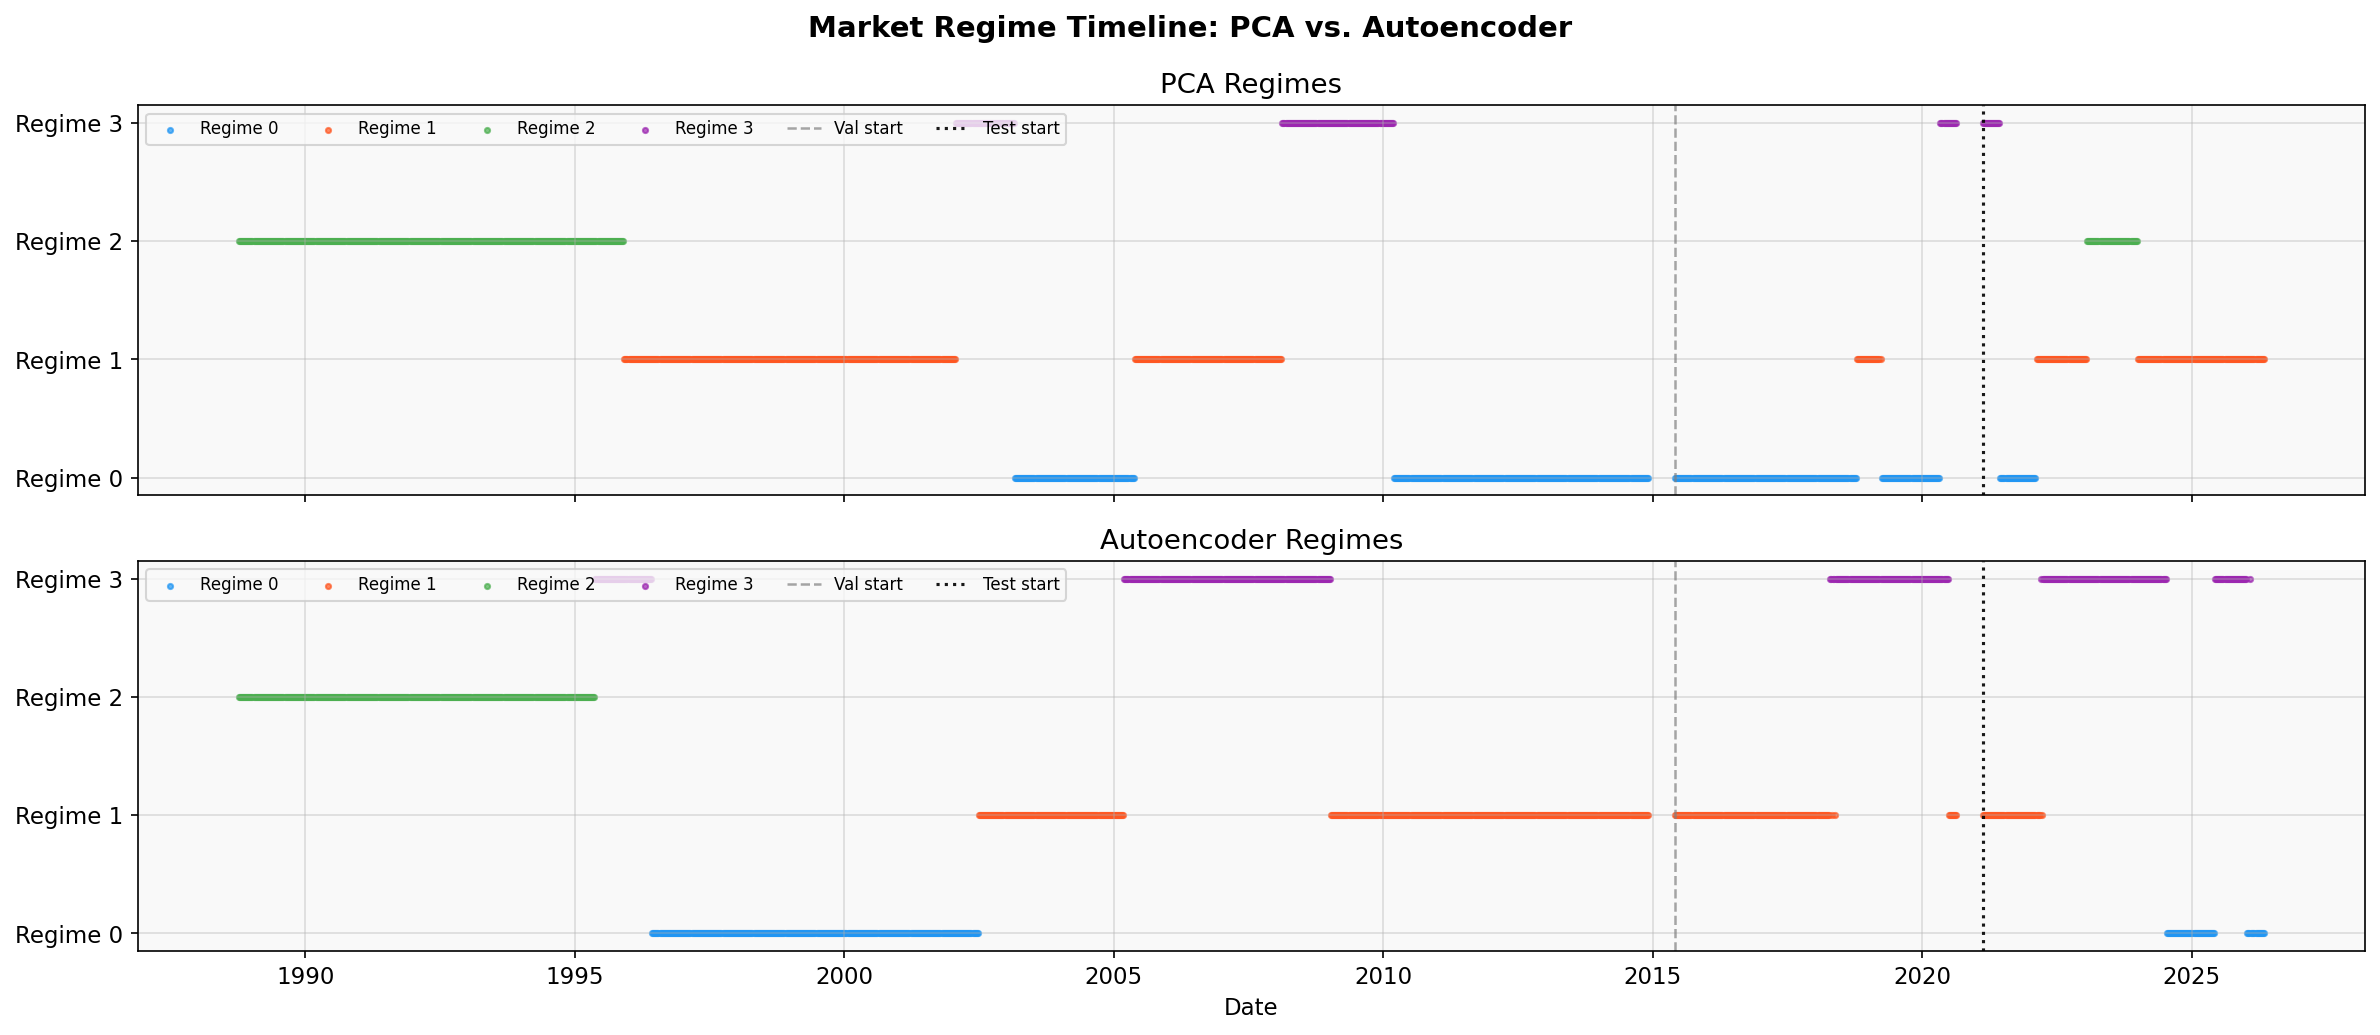
\includegraphics[width=\textwidth]{05_regime_timeline.png}
  \caption{Regime timeline for PCA (top) and the autoencoder (bottom) across the
  full sample. Dashed and dotted lines mark the validation and test boundaries.}
  \label{fig:timeline}
\end{figure*}

A notable observation concerns out-of-sample regime coverage. While the
autoencoder uses all four regimes on the training set, the validation window
(2014--2020) populates only two of them, and the test window (2020--2026) only
three, with regime~2 (the inflationary state) entirely absent out of sample. As
the ablation in Section~\ref{sec:ablation} shows, this coverage gap persists
across latent widths --- the validation period collapses to two regimes whether
the bottleneck is 2- or 32-dimensional --- so it reflects a genuine structural
shift in the out-of-sample periods rather than insufficient model capacity. The
out-of-sample windows simply do not exercise the full regime vocabulary learned
in training. This is consistent with the elevated test reconstruction loss
(Table~\ref{tab:recon}) and with the deterioration of the trading rule out of
sample reported in Section~\ref{sec:strategy}.

\subsection{Regime-Conditioned Trading Strategy}
\label{sec:strategy}

To assess whether the identified regimes carry economic value beyond
descriptive interpretation, we construct a simple regime-conditioned trading
rule and evaluate it strictly out of sample. For each window we compute the
realized one-week-forward return of the market factor (\texttt{\_MKT}), so
window $i$'s forward return is the new observation introduced by window
$i+1$. The trading rule itself is derived using only the training partition:
for each of the four autoencoder regimes we compute the average forward return
in training (Table~\ref{tab:regime-returns}), rank the regimes accordingly, and
assign a fixed position to each regime, long the highest-return regime, short
the lowest-return regime, and flat for the two intermediate regimes. This
position map is then frozen and applied unchanged to the validation and test
partitions, so no information from outside the training period is used to
construct the rule.

\begin{table}[h]
\centering
\caption{Average one-week-forward return by regime (training set, standardized units) and the resulting position.}
\label{tab:regime-returns}
\begin{tabular}{ccc}
\toprule
Regime & Mean forward return (train) & Position \\
\midrule
1 & $+0.032$ & Long ($+1$) \\
2 & $+0.030$ & Flat ($0$) \\
0 & $-0.022$ & Flat ($0$) \\
3 & $-0.069$ & Short ($-1$) \\
\bottomrule
\end{tabular}
\end{table}

\begin{table}[h]
\centering
\caption{Strategy performance by split. Sharpe ratios are annualized
(weekly returns, $\sqrt{52}$ scaling) and computed on standardized returns;
IC is the Spearman rank correlation between the assigned position and the
realized forward return.}
\label{tab:strategy-results}
\begin{tabular}{lccc}
\toprule
Split & Strategy Sharpe & Buy-and-hold Sharpe & IC \\
\midrule
Train (in-sample) & 0.23 & 0.00 & 0.03 \\
Validation (OOS) & 0.13 & $-0.02$ & $-0.02$ \\
Test (OOS) & $-0.28$ & 0.07 & $-0.04$ \\
\bottomrule
\end{tabular}
\end{table}

The strategy is profitable in sample, with a Sharpe ratio of $0.23$ and a
positive IC of $0.03$, both consistent with the ranking used to construct the
rule by design. Out of sample the picture is mixed and ultimately negative: the
validation Sharpe ratio is positive but modest ($0.13$) and IC is slightly
negative ($-0.02$), but on the test partition the strategy loses money relative
to a flat position, with a Sharpe ratio of $-0.28$ and an IC indistinguishable
from zero. A simple buy-and-hold benchmark over the same out-of-sample period
slightly outperforms the regime-conditioned strategy on test. While the expanded
16-dimensional architecture successfully resolved the validation mode collapse,
the strategy's failure in the test set supports the theory that the post-2020
era represents an unprecedented regime shift that fundamentally altered market behavior.

We therefore do not consider the current regime signal a reliable basis for
investment on its own. The in-sample relationship between regime and forward
return is economically sensible (the regime associated with elevated
unemployment and volatility precedes the lowest forward returns, and the
low-volatility regime precedes the highest), but it does not survive the
out-of-sample test in its present form. A plausible path toward an investable
strategy would combine the regime signal with additional confirming
indicators, widen the latent space so the encoder is less prone to collapsing
distinct periods into a single regime, or use the regime as one input among
several in a more conventional return-forecasting model rather than as a
standalone signal.

\subsection{Robustness to the Choice of Input Signals}
\label{sec:signals}

A natural objection is that the out-of-sample failure of the regime signal might
be an artifact of the particular 30-feature input set rather than a property of
regime-conditioned trading itself. To test this, we retrain the autoencoder under
an identical architecture, optimizer, seed, and clustering protocol on three
different input feature sets and re-run the full pipeline of
Section~\ref{sec:strategy} --- training, clustering, rule derivation on training
data only, and out-of-sample evaluation --- separately for each:
\begin{itemize}
  \item \textbf{Set A (macro cycle, 10 features):} GDP, CPI, M2, unemployment,
        consumer confidence, and the principal interest-rate and yield series.
  \item \textbf{Set B (risk and sentiment, 10 features):} the equity market
        factor, the MOVE volatility index, dividend yield, yield-spread stress,
        and the traded price series (credit, Treasury, oil, gold, dollar).
  \item \textbf{Full (all 30 features):} the main paper configuration.
\end{itemize}
Because each model is trained from scratch with the same seed and the position
rule is re-derived from training data only, the three configurations in
Table~\ref{tab:signals} are directly comparable.

\begin{table*}[t]
\centering
\caption{Robustness of the regime-conditioned strategy to the choice of input
signals. Each autoencoder is retrained from scratch under identical settings on
a different feature subset; the long/flat/short rule is re-derived on training
data only and evaluated out of sample. Sharpe ratios are annualized; the test IC
is the Spearman rank correlation between the assigned position and the realized
forward return on the test split.}
\label{tab:signals}
\begin{tabular}{lccccccc}
\toprule
 & \multicolumn{3}{c}{Reconstruction MSE} & \multicolumn{3}{c}{Strategy Sharpe} & Test \\
\cmidrule(lr){2-4}\cmidrule(lr){5-7}
Signal set & Train & Val & Test & Train & Val & Test & IC \\
\midrule
Set A (macro, 10 feat.)          & 0.029 & 0.448 & 0.973 & 0.30 & $-0.62$           & $-0.05$ & $-0.00$ \\
Set B (risk/sentiment, 10 feat.) & 0.619 & 0.629 & 0.653 & 0.44 & $-0.44$           & $-0.33$ & $-0.05$ \\
Full (all 30 feat.)              & 0.303 & 0.612 & 1.197 & 0.33 & $\phantom{-}0.00$ & $-0.28$ & $-0.07$ \\
\bottomrule
\end{tabular}
\end{table*}

Two patterns stand out. First, reconstruction quality is highly sensitive to the
feature mix. The macro-only Set~A reconstructs its smooth, slow-moving inputs
almost perfectly in sample (train MSE $0.029$) but degrades sharply out of sample
(test MSE $0.973$), whereas the noisier risk/sentiment Set~B reconstructs less
well in sample (train MSE $0.619$) yet stays nearly flat across splits
($0.619 \rightarrow 0.653$), reflecting the greater stationarity of return- and
volatility-based features. Second, and more importantly, the economic verdict is
unchanged regardless of the input set: every configuration is profitable in sample
(train Sharpe $0.30$--$0.44$) but loses money out of sample, with a negative test
Sharpe in all three cases.\footnote{The Full row is retrained inline under the
comparison protocol rather than loaded from the handoff checkpoint of
Section~\ref{sec:strategy}; its in-sample Sharpe therefore differs slightly from
Table~\ref{tab:strategy-results} ($0.33$ versus $0.23$), but the out-of-sample
test Sharpe ($-0.28$) is reproduced.} The out-of-sample breakdown is therefore not
an artifact of one particular feature selection --- it is a robust property of
regime-conditioned trading over this sample, consistent with the structural shift
documented in Sections~\ref{sec:ablation} and~\ref{sec:strategy}.

\subsection{Discussion}

Both methods recover interpretable market structure, but the moderate agreement
between them is the central finding: the autoencoder and PCA do not simply
reproduce one another. Because 16 PCA components retain less than three-quarters
of the variance, part of the disagreement is attributable to information that the
linear projection discards and the nonlinear encoder retains. We adopt a
16-dimensional bottleneck because it minimizes out-of-sample reconstruction loss
(Section~\ref{sec:ablation}); it should be stressed, however, that capacity alone
does not fix the out-of-sample regime collapse, which the ablation shows persists
at every latent width. A second, sobering observation is that the nonlinear
autoencoder only moderately outperforms the linear PCA baseline: a large share of
the regime structure is in fact linear, and the additional value of the neural
network over PCA in this setting, while real, is modest.

The trading strategy in Section~\ref{sec:strategy} sharpens this point with an
economic test rather than a purely representational one. The in-sample
regime-return relationship is exactly what the feature profiles in
Table~\ref{tab:regimes} would predict, which is reassuring evidence that the
unsupervised regimes are not arbitrary. However, the strategy's failure to
generalize to the test period highlights the massive structural break introduced
by post-2020 market conditions. Section~\ref{sec:signals} shows that this failure
is robust to the choice of input signals: macro-only, risk/sentiment-only, and
the full feature set all yield strategies that are profitable in sample yet post a
negative test Sharpe, so the breakdown is a property of the regime signal over
this period rather than of one particular feature selection. This suggests that
while 16 dimensions are enough
to capture the structure of the historical training period, historical models of
any capacity struggle to generalize across true, unprecedented regime shifts.

\section{Limitations}

The study has several limitations. Results depend on the chosen dataset and
sample period and are sensitive to hyperparameter choices, particularly the
latent dimensionality and the number of clusters. K-Means assumes roughly convex,
comparably sized clusters, which may not match the true regime geometry, and the
choice of four clusters is motivated by interpretability rather than by an
internal cluster-validity optimum (Section~\ref{sec:strategy}). The latent
dimensions are not directly interpretable as economic quantities.

Three further caveats deserve emphasis. First, the windows overlap heavily: with
a 26-week window and a one-week stride, consecutive inputs share 25 of 26 weeks,
so the $1{,}365$ training windows correspond to far fewer statistically
independent macroeconomic episodes. Effective sample size is therefore much
smaller than the row count suggests, which inflates the apparent stability of the
regimes and makes any estimated regime--return relationship prone to overfitting.
Second, the autoencoder is trained purely to minimize reconstruction error;
nothing in the objective encourages the latent space to separate \emph{future}
returns or even to be well suited to clustering, so the downstream regimes are a
by-product of compression rather than an optimized target. Third, the Sharpe
ratios and information coefficients in Section~\ref{sec:strategy} are computed on
\emph{standardized} market returns rather than raw percentage returns; the
sign-, ranking-, and correlation-based conclusions are unaffected, but the Sharpe
magnitudes are not directly comparable to those of a real percentage-return
strategy.

Finally, the regime-conditioned strategy of Section~\ref{sec:strategy} is
intentionally simple (a fixed long/flat/short rule with no position sizing,
transaction costs, or risk management) and is intended as a diagnostic of whether
the regimes carry directional information, not as a deployable strategy; its
out-of-sample underperformance should be interpreted in that light rather than as
a definitive verdict on regime-based investing in general.

\section{Future Work}

Future extensions include testing alternative architectures such as LSTM or
variational autoencoders, adding a clustering-aware or contrastive term to the
training objective so the latent space is optimized for regime separation rather
than reconstruction alone, incorporating additional asset classes and
macroeconomic variables, and exploring dynamic or online regime detection. On the trading side, natural next steps include adding position
sizing and transaction costs to the regime-conditioned strategy, combining the
regime signal with complementary predictors rather than trading it in
isolation, and retraining the autoencoder periodically (e.g., with an
expanding or rolling window) so that the latent space and the implied regimes
can adapt to new data instead of remaining fixed at the original training
boundary.

\section{Conclusion}

We presented an unsupervised framework for market regime detection that combines
a 16-dimensional autoencoder with K-Means clustering and benchmarks it against
a PCA projection of equal dimensionality. The autoencoder learns a compact
representation that reconstructs the data well in sample and identifies four
regimes corresponding to recognizable market and economic environments. The
moderate agreement with PCA (ARI $0.52$, NMI $0.58$) indicates that nonlinear
representation learning captures structure beyond what a 16-component linear
projection can express --- but the gain over the linear baseline is modest, and
much of the recovered regime structure is in fact linear. Out of sample the
limits are clear: reconstruction loss rises sharply, the validation and test
periods populate only part of the regime vocabulary, and a regime-conditioned
trading rule that is profitable in sample fails to beat a buy-and-hold benchmark
on the test period. Taken together, the results position the autoencoder as a
useful descriptive lens on historical market structure rather than a
ready-to-deploy investment signal, and they underscore the difficulty of
generalizing any historically trained regime model across genuinely unprecedented
market shifts.

To directly address whether the detected regimes are an appropriate basis for
investment, we backtested a regime-conditioned long/short strategy fixed from
training data alone. The answer, based on the current 16-dimensional
autoencoder, is no: the strategy is profitable and economically coherent in
sample (Sharpe $0.23$) but loses to a flat benchmark out of sample (Sharpe
$-0.28$ on test), with an information coefficient that is indistinguishable
from zero in the most recent period. We would not recommend deploying this
regime signal as a stand-alone trading strategy in its present form. The result
is nonetheless informative: the in-sample regime-return relationship is
economically sensible, and the out-of-sample failure is consistent with the massive
structural break seen in the 2020--2026 data. This suggests that while representation
learning can effectively characterize historical environments, building a strategy
that generalizes to unprecedented environments may require complementary predictors
or dynamic adaptation rather than just wider bottlenecks.
Overall, the results support representation learning as a useful, if not
yet decisive, tool for characterizing financial market regimes.

\bibliographystyle{IEEEtran}
\bibliography{mybibfile}

\end{document}